\chapter{Trabajos Relacionados}
\section{Consideraciones Iniciales}
En este capítulo se discute... 
\section{Minería Visual de Datos}

Cuando se hace análisis de datos primero se especifica ciertos parámetros para restringir el espacio de búsqueda; de esta forma la minería de datos trabaja de forma automática siguiendo un algoritmo (matemático, estadístico o de inteligencia artificial), finalmente los patrones son encontrados por este algoritmo para luego ser presentados como resultados en pantalla. Dado que existe gran cantidad de patrones generados por el algoritmo de minería de datos automática en forma textual, es casi imposible para el ser humano interpretar y evaluar el patrón en detalle para extraer conocimientos interesantes y características generales. Por otra parte la visualización de información es un estudio de representaciones (interactivas) visuales de datos para reforzar la cognición humana. Estas dos estrategias de de tratamiento de información (minería de datos y visualización de información) pueden llegar a ser complementarias y coexistir en la búsqueda de soluciones para la interpretación de un conjunto de datos complejos o naturales. Por lo tanto, para que la minería de datos sea efectiva es importante incluir a los humanos en el proceso de exploración de datos y combinar la flexibilidad, creatividad y el conocimiento general de la persona con la gran capacidad de almacenamiento y procesamiento de las computadoras de hoy en día. Tal área es denominada \textit{Minería Visual de Datos} \cite{wong1999guest}.

La minería visual de datos tiene como objetivo la integración del humano en el proceso de minería de datos, y la aplicación de las capacidades perceptivas de los humanos para el análisis de grandes conjuntos disponibles. la presentación de los datos en un formulario gráfico en interactivo a menudo fomenta la formación y la validación de nuevas hipótesis, para una buena toma de decisiones por consiguiente una buena resolución de los problemas. Con la visualización obtenemos una la formación y visión de estas hipótesis, la verificación de estas hipótesis se puede realizar también mediante la vía de visualización, pero lo mas conveniente es que vaya respaldado con algunas técnicas automáticas de análisis matemático, estadístico o aprendizaje maquina. 

Ankerst \cite{ankerst2001visual} clasifica en tres enfoques comunes la integración del humano en el proceso de exploración de datos como se muestra en la figura \ref{fig:VDM} :
\begin{itemize}
	\item \textbf{Visualización Anterior.} La visualización de información se realiza antes de que el algoritmo de minería de datos sea ejecutado, con la interacción se tiene un control total sobre el espacio de búsqueda. 
	\item \textbf{Visualización Posterior.} El algoritmo de minería de datos automática se ejecuta primero para la extracción de patrones y estos son mostrados por la visualización, se puede hacer re-calibraciones para posteriores exploraciones, esto con el objetivo de introducir otros parámetros y obtener mejores resultados.
	\item \textbf{Visualización fuertemente Integrado.} Un algoritmo de minería de datos automática realiza un análisis de los datos, pero no produce los resultados finales. Una técnica de visualización se utiliza para presentar los resultados  del proceso de exploración de datos. La combinación de algunos algoritmos de minería de datos automáticos y técnicas de visualización permite  realizar una retroalimentación en el proceso de exploración. De esta forma se permite al usuario entender y llevar mejor el proceso de exploración; trabajar con datos con alto contenido de ruido; no se necesita de alto conocimiento de los algoritmos matemáticos o estadísticos; permite una visión cualitativa de los datos para su posterior análisis cuantitativo.
\end{itemize}

En resumen la minería visual de datos se compone por un lado la minería de datos que son la generación o descubriendo de patrones a partir de un conjunto de datos basándose en técnicas matemáticas, estadísticas o de inteligencia artificial y por otro lado las técnicas de visualización que son la generación de imágenes o de representaciones gráficas a partir de estos datos.
\begin{figure}[!h]
\centering
\includegraphics[width=\columnwidth]{figs/VDM.pdf}%
\caption{Vista general de los diferentes enfoques de la integración de los humanos en el proceso de exploración de datos.}%
\label{fig:VDM}%
\end{figure}

\section{Visualización de Información}
La visualización de información \cite{card1999readings} es el uso de representaciones visuales e interactivas de datos para amplificar la cognición. Esto significa que los datos son transformados en una imagen. La imagen puede ser cambiado por los usuarios a media que se vaya trabajando con él. Esta interacción es importante, ya que permite una constante redefinición de objetivos cuando una nueva visión de los datos se han obtenido.
Esta área esta ampliando su espectro debido al desarrollo de la visualización en computadoras en tiempo real. Este medio es promisorio porque acrecienta los recursos del humano en la forma de procesamiento perceptual, permite reducir el tiempo de búsqueda de información, permite mejorar el reconocimiento de patrones, permite el uso de  inferencia y monitoreo perceptual en un medio manipulable e interactivo.
Dentro de las subáreas fundamentales se encuentran la visualización de datos multidimensionales, el cual estudiaremos por la importancia dentro del desarrollo del presente trabajo.
\section{Visualización de Datos Multidimensionales}
		\subsection{Proyecciones Multidimensionales}
		\subsection{Métricas de medición de calidad de una proyección}
		\subsection{Técnicas de visualización Radial}
		\subsection{Radviz}
		\subsection{Star Coordinates}
\section{Consideraciones Finales}
